\documentclass[apuntes,doscolumnas]{uc3mmaster}
\titulo{Transformación evolutiva de atributos: forma, relevancia, reducción y síntesis}\asignatura{IA de Inspiración Biológica}\tipo{Apuntes}
\autor{Andrea López Salazar}{}
\usepackage{lipsum}
\usepackage{multirow}
\definecolor{azulm}{HTML}{2E6DB4}\definecolor{naranjam}{HTML}{D9731A}
\definecolor{verdem}{HTML}{2F9467}\definecolor{grism}{HTML}{5A6772}
% Generado por analisis.py: NO editar a mano.
\newcommand{\nDatasets}{12}
\newcommand{\nParticiones}{5}
\newcommand{\nCasos}{60}
\newcommand{\relRL}{0{,}96}
\newcommand{\cambioRL}{$-$4{,}4\,\%}
\newcommand{\casosRL}{36/60}
\newcommand{\dsRL}{7/12}
\newcommand{\pRL}{$1{,}000$}
\newcommand{\cambioVsEstRL}{$-$2{,}6\,\%}
\newcommand{\dsVsEstRL}{6/12}
\newcommand{\pVsEstRL}{$1{,}000$}
\newcommand{\peorDsRL}{$+$20{,}9\,\%}
\newcommand{\relKNN}{0{,}76}
\newcommand{\cambioKNN}{$-$24{,}3\,\%}
\newcommand{\casosKNN}{56/60}
\newcommand{\dsKNN}{12/12}
\newcommand{\pKNN}{$0{,}004$}
\newcommand{\cambioVsEstKNN}{$-$13{,}6\,\%}
\newcommand{\dsVsEstKNN}{10/12}
\newcommand{\pVsEstKNN}{$0{,}048$}
\newcommand{\peorDsKNN}{$-$0{,}4\,\%}
\newcommand{\relArbol}{1{,}00}
\newcommand{\cambioArbol}{$+$0{,}1\,\%}
\newcommand{\casosArbol}{34/60}
\newcommand{\dsArbol}{7/12}
\newcommand{\pArbol}{$1{,}000$}
\newcommand{\cambioVsEstArbol}{$+$0{,}1\,\%}
\newcommand{\dsVsEstArbol}{7/12}
\newcommand{\pVsEstArbol}{$1{,}000$}
\newcommand{\peorDsArbol}{$+$5{,}0\,\%}
\newcommand{\relRF}{1{,}00}
\newcommand{\cambioRF}{$+$0{,}5\,\%}
\newcommand{\casosRF}{27/60}
\newcommand{\dsRF}{5/12}
\newcommand{\pRF}{$1{,}000$}
\newcommand{\cambioVsEstRF}{$+$0{,}5\,\%}
\newcommand{\dsVsEstRF}{5/12}
\newcommand{\pVsEstRF}{$1{,}000$}
\newcommand{\peorDsRF}{$+$4{,}1\,\%}
\newcommand{\cambioSintRL}{$-$1{,}3\,\%}
\newcommand{\pSintRL}{$0{,}705$}
\newcommand{\dsSintRL}{7/12}
\newcommand{\relSintRL}{0{,}99}
\newcommand{\cambioSintKNN}{$-$0{,}3\,\%}
\newcommand{\pSintKNN}{$0{,}705$}
\newcommand{\dsSintKNN}{7/12}
\newcommand{\relSintKNN}{1{,}00}
\newcommand{\cambioSintArbol}{$+$0{,}3\,\%}
\newcommand{\pSintArbol}{$1{,}000$}
\newcommand{\dsSintArbol}{7/12}
\newcommand{\relSintArbol}{1{,}00}
\newcommand{\cambioSintRF}{$-$0{,}1\,\%}
\newcommand{\pSintRF}{$1{,}000$}
\newcommand{\dsSintRF}{7/12}
\newcommand{\relSintRF}{1{,}00}
\newcommand{\cambioRedRL}{$+$1{,}8\,\%}
\newcommand{\pRedRL}{$0{,}380$}
\newcommand{\dsRedRL}{5/12}
\newcommand{\relRedRL}{1{,}02}
\newcommand{\cambioRedKNN}{$+$1{,}0\,\%}
\newcommand{\pRedKNN}{$0{,}330$}
\newcommand{\dsRedKNN}{4/12}
\newcommand{\relRedKNN}{1{,}01}
\newcommand{\cambioRedArbol}{$+$1{,}4\,\%}
\newcommand{\pRedArbol}{$0{,}330$}
\newcommand{\dsRedArbol}{3/12}
\newcommand{\relRedArbol}{1{,}01}
\newcommand{\cambioRedRF}{$+$2{,}8\,\%}
\newcommand{\pRedRF}{$0{,}049$}
\newcommand{\dsRedRF}{1/12}
\newcommand{\relRedRF}{1{,}03}
\newcommand{\dimMedia}{83\,\%}
\newcommand{\fracEliminados}{22\,\%}
\newcommand{\dimMin}{38\,\%}
\newcommand{\dimMax}{92\,\%}
\newcommand{\mMedia}{0{,}4}
\newcommand{\fracConSintesis}{25\,\%}
\newcommand{\tauMediana}{0{,}18}
\newcommand{\casosNmenosUno}{38/60}
\newcommand{\wLat}{2{,}91}
\newcommand{\wLon}{2{,}85}
\newcommand{\wPop}{0{,}03}
\newcommand{\wInc}{0{,}41}
\newcommand{\fracApagados}{10\,\%}
\newcommand{\nCompCasos}{60}
\newcommand{\compMLKRRL}{$-$1{,}8\,\%}
\newcommand{\compMLKRKNN}{$-$22{,}5\,\%}
\newcommand{\compMLKRArbol}{$+$2{,}0\,\%}
\newcommand{\compMLKRRF}{$+$2{,}6\,\%}
\newcommand{\rangoMLKR}{5{,}7}
\newcommand{\compPGRL}{$-$15{,}7\,\%}
\newcommand{\compPGKNN}{$-$18{,}0\,\%}
\newcommand{\compPGArbol}{$+$0{,}7\,\%}
\newcommand{\compPGRF}{$+$0{,}8\,\%}
\newcommand{\rangoPG}{4{,}6}
\newcommand{\compYJMVRL}{$+$2{,}4\,\%}
\newcommand{\compYJMVKNN}{$-$14{,}5\,\%}
\newcommand{\compYJMVArbol}{$+$1{,}5\,\%}
\newcommand{\compYJMVRF}{$+$1{,}7\,\%}
\newcommand{\rangoYJMV}{5{,}0}
\newcommand{\compCuantRL}{$+$8{,}1\,\%}
\newcommand{\compCuantKNN}{$-$11{,}8\,\%}
\newcommand{\compCuantArbol}{$+$0{,}1\,\%}
\newcommand{\compCuantRF}{$+$0{,}0\,\%}
\newcommand{\rangoCuant}{6{,}4}
\newcommand{\compEstPCARL}{$-$1{,}8\,\%}
\newcommand{\compEstPCAKNN}{$-$12{,}4\,\%}
\newcommand{\compEstPCAArbol}{$-$0{,}6\,\%}
\newcommand{\compEstPCARF}{$-$1{,}9\,\%}
\newcommand{\rangoEstPCA}{4{,}6}
\newcommand{\compPCAnoventaRL}{$+$0{,}6\,\%}
\newcommand{\compPCAnoventaKNN}{$-$10{,}4\,\%}
\newcommand{\compPCAnoventaArbol}{$+$19{,}3\,\%}
\newcommand{\compPCAnoventaRF}{$+$17{,}9\,\%}
\newcommand{\rangoPCAnoventa}{8{,}1}
\newcommand{\compPCAcvRL}{$-$1{,}0\,\%}
\newcommand{\compPCAcvKNN}{$-$12{,}0\,\%}
\newcommand{\compPCAcvArbol}{$+$18{,}7\,\%}
\newcommand{\compPCAcvRF}{$+$15{,}1\,\%}
\newcommand{\rangoPCAcv}{7{,}4}
\newcommand{\compPsrRL}{$-$6{,}1\,\%}
\newcommand{\compPsrKNN}{$-$25{,}0\,\%}
\newcommand{\compPsrArbol}{$-$1{,}1\,\%}
\newcommand{\compPsrRF}{$-$2{,}3\,\%}
\newcommand{\rangoPsr}{3{,}2}
\newcommand{\compPRL}{$-$4{,}4\,\%}
\newcommand{\compPKNN}{$-$24{,}3\,\%}
\newcommand{\compPArbol}{$+$0{,}1\,\%}
\newcommand{\compPRF}{$+$0{,}5\,\%}
\newcommand{\rangoP}{4{,}7}
\newcommand{\mejorAlt}{estándar + PCA}
\newcommand{\rangoMejorAlt}{4{,}6}
\newcommand{\nReps}{10}
\newcommand{\vMedia}{0{,}80}
\newcommand{\vFracUno}{22\,\%}
\newcommand{\nSintMedia}{3{,}9}
\newcommand{\ctrlIniAleat}{$+$0{,}6\,\%}
\newcommand{\pCtrlIniAleat}{$1{,}000$}
\newcommand{\ctrlIniAleatRL}{$+$1{,}7\,\%}
\newcommand{\ctrlSigmaBajo}{$+$0{,}5\,\%}
\newcommand{\pCtrlSigmaBajo}{$1{,}000$}
\newcommand{\ctrlSigmaBajoRL}{$-$0{,}1\,\%}
\newcommand{\ctrlSigmaAlto}{$+$0{,}9\,\%}
\newcommand{\pCtrlSigmaAlto}{$1{,}000$}
\newcommand{\ctrlSigmaAltoRL}{$-$0{,}4\,\%}
\newcommand{\ctrlPobDoble}{$+$0{,}2\,\%}
\newcommand{\pCtrlPobDoble}{$1{,}000$}
\newcommand{\ctrlPobDobleRL}{$-$0{,}2\,\%}
\newcommand{\nAblCasos}{24}
\newcommand{\ctrlPesos}{$+$2{,}2\,\%}
\newcommand{\ctrlPesosRL}{$+$6{,}5\,\%}
\newcommand{\pCtrlPesos}{$0{,}424$}
\newcommand{\ctrlExp}{$+$10{,}0\,\%}
\newcommand{\ctrlExpRL}{$+$2{,}2\,\%}
\newcommand{\pCtrlExp}{$0{,}012$}
\newcommand{\ctrlAleat}{$+$6{,}2\,\%}
\newcommand{\ctrlAleatRL}{$+$3{,}0\,\%}
\newcommand{\pCtrlAleat}{$0{,}012$}
\newcommand{\ctrlMI}{$+$14{,}9\,\%}
\newcommand{\ctrlMIRL}{$+$6{,}8\,\%}
\newcommand{\pCtrlMI}{$0{,}012$}
\newcommand{\ctrlYJMI}{$+$11{,}0\,\%}
\newcommand{\ctrlYJMIRL}{$+$10{,}3\,\%}
\newcommand{\pCtrlYJMI}{$0{,}014$}
\newcommand{\nCtrlCasos}{24}
\newcommand{\rangoCeroR}{$+$2{,}2\,\%}
\newcommand{\pRangoCero}{$1{,}000$}
\newcommand{\dsPeorRangoCero}{7}
\newcommand{\rangoUnoR}{$+$0{,}3\,\%}
\newcommand{\pRangoUno}{$1{,}000$}
\newcommand{\dsPeorRangoUno}{6}
\newcommand{\rangoCuatroR}{$+$0{,}5\,\%}
\newcommand{\pRangoCuatro}{$1{,}000$}
\newcommand{\dsPeorRangoCuatro}{7}
\newcommand{\rangoOchoR}{$+$1{,}7\,\%}
\newcommand{\pRangoOcho}{$0{,}256$}
\newcommand{\dsPeorRangoOcho}{9}
\newcommand{\bordeUno}{11\,\%}
\newcommand{\bordeDos}{7\,\%}
\newcommand{\bordeCuatro}{8\,\%}
\newcommand{\bordeOcho}{5\,\%}
\newcommand{\nRango}{24}
\newcommand{\mleFueraDos}{24\,\%}
\newcommand{\nAlgCasos}{24}
\newcommand{\rangoCMA}{1{,}9}
\newcommand{\algMejor}{CMA-ES}
\newcommand{\algKNNcma}{$-$25{,}7\,\%}
\newcommand{\algKNNaleat}{$-$21{,}0\,\%}
\newcommand{\algKNNmin}{$-$24{,}8\,\%}
\newcommand{\algKNNmax}{$-$23{,}3\,\%}
\newcommand{\segMediana}{191}
\newcommand{\segMax}{243}
\newcommand{\msPorEval}{191}
\newcommand{\segMLKR}{16{,}8}
\newcommand{\segPG}{6{,}1}
\newcommand{\segYJMV}{0{,}6}
\newcommand{\popMin}{11}
\newcommand{\popMax}{13}
\newcommand{\muMin}{5}
\newcommand{\muMax}{6}
\newcommand{\muEffMin}{3{,}4}
\newcommand{\muEffMax}{4{,}0}
\newcommand{\genMin}{77}
\newcommand{\genMax}{91}
\newcommand{\nParadaPresupuesto}{12}
\newcommand{\nParadaTotal}{12}
\newcommand{\evalMejorMediana}{971}
\newcommand{\evalMejorMin}{658}
\newcommand{\mejoraFitnessMediana}{$-$12{,}1\,\%}
\newcommand{\sigmaFinMin}{0{,}007}
\newcommand{\sigmaFinMax}{0{,}06}
\newcommand{\cribSelRL}{$-$2{,}5\,\%}
\newcommand{\cribSelKNN}{$-$23{,}9\,\%}
\newcommand{\cribSelArbol}{$+$0{,}1\,\%}
\newcommand{\cribSelRF}{$+$0{,}8\,\%}
\newcommand{\cribDimSel}{72\,\%}
\newcommand{\cribFijoRL}{$-$5{,}4\,\%}
\newcommand{\cribFijoKNN}{$-$25{,}0\,\%}
\newcommand{\cribFijoArbol}{$-$0{,}5\,\%}
\newcommand{\cribFijoRF}{$+$0{,}0\,\%}
\newcommand{\cribDimFijo}{89\,\%}
\newcommand{\cribPcaRL}{$-$2{,}7\,\%}
\newcommand{\cribPcaKNN}{$-$23{,}9\,\%}
\newcommand{\cribPcaArbol}{$+$0{,}8\,\%}
\newcommand{\cribPcaRF}{$+$1{,}9\,\%}
\newcommand{\cribDimPca}{70\,\%}
\newcommand{\cribFijoNoReduce}{27/60}
% Generado por analisis.py: filas de las tablas (una macro por tabla).
\newcommand{\filasPrincipal}{%
R. lineal & 0{,}98 & 0{,}94 & \textbf{0{,}96} & 7/12 & $1{,}000$ & $-$2{,}6\,\%\\
KNN & 0{,}88 & 0{,}75 & \textbf{0{,}76} & 12/12 & $0{,}004$ & $-$13{,}6\,\%\\
Árbol & 1{,}00 & 0{,}99 & \textbf{1{,}00} & 7/12 & $1{,}000$ & $+$0{,}1\,\%\\
RF & 1{,}00 & 0{,}98 & \textbf{1{,}00} & 5/12 & $1{,}000$ & $+$0{,}5\,\%\\
}
\newcommand{\filasDimension}{%
diabetes & 10 & 8{,}0 & 0{,}6 & 8{,}6 & 0{,}46\\
concrete & 8 & 6{,}6 & 0{,}0 & 6{,}6 & 0{,}47\\
stock & 9 & 7{,}6 & 0{,}4 & 8{,}0 & 0{,}30\\
space\_ga & 6 & 3{,}8 & 0{,}4 & 4{,}2 & 0{,}09\\
sulfur & 6 & 5{,}0 & 0{,}0 & 5{,}0 & 0{,}01\\
wine\_quality & 11 & 9{,}6 & 0{,}2 & 9{,}8 & 0{,}41\\
kin8nm & 8 & 7{,}0 & 0{,}0 & 7{,}0 & 0{,}34\\
bank8FM & 8 & 6{,}8 & 0{,}2 & 7{,}0 & 0{,}05\\
puma8NH & 8 & 2{,}2 & 2{,}4 & 4{,}6 & 1{,}83\\
house\_8L & 8 & 7{,}0 & 0{,}0 & 7{,}0 & 0{,}12\\
cpu\_small & 12 & 10{,}8 & 0{,}2 & 11{,}0 & 0{,}19\\
california & 8 & 6{,}6 & 0{,}0 & 6{,}6 & 0{,}02\\
}
\newcommand{\filasComparativa}{%
estándar & 0{,}98 & 0{,}88$^*$ & 1{,}00 & 1{,}00 & 5{,}3 & 1{,}00\\
YJ máx.\ verosimilitud & 1{,}02 & 0{,}85$^*$ & 1{,}01 & 1{,}02 & 5{,}0 & 1{,}00\\
cuantiles & 1{,}08 & 0{,}88$^*$ & 1{,}00 & 1{,}00 & 6{,}4 & 1{,}00\\
solo PCA (95\,\%) & 1{,}01 & 0{,}90$^*$ & 1{,}19$^*$ & 1{,}18$^*$ & 8{,}1 & 0{,}79\\
solo PCA (\% por VC) & 0{,}99 & 0{,}88$^*$ & 1{,}19$^*$ & 1{,}15 & 7{,}4 & 0{,}91\\
estándar + su PCA & 0{,}98 & 0{,}88$^*$ & 0{,}99 & 0{,}98 & 4{,}6 & 2{,}00\\
MLKR & 0{,}98 & 0{,}78 & 1{,}02 & 1{,}03 & 5{,}7 & 1{,}00\\
PG (gplearn) & \textbf{0{,}84} & 0{,}82$^*$ & 1{,}01 & 1{,}01 & 4{,}6 & 2{,}00\\
$P$ sin reducir & 0{,}94 & \textbf{0{,}75} & \textbf{0{,}99} & \textbf{0{,}98} & 3{,}2 & 2{,}00\\
\textbf{$P$} & 0{,}96 & 0{,}76 & 1{,}00 & 1{,}00 & 4{,}7 & 0{,}83\\
}
\newcommand{\filasAblacion}{%
\multicolumn{4}{@{}l}{\emph{Piezas}}\\
\quad solo pesos ($\lambda=1$) & $+$2{,}2\,\% & $+$6{,}5\,\% & $-$0{,}1\,\%\\
\quad solo exponentes ($w=1$) & $+$10{,}0\,\%$^*$ & $+$2{,}2\,\% & $+$0{,}4\,\%\\
\midrule
\multicolumn{4}{@{}l}{\emph{Sin búsqueda}}\\
\quad pesos por inf.\ mutua & $+$14{,}9\,\%$^*$ & $+$6{,}8\,\% & $+$3{,}6\,\%\\
\quad YJ (MV) + pesos inf.\ mutua & $+$11{,}0\,\% & $+$10{,}3\,\% & $+$3{,}6\,\%\\
\midrule
\multicolumn{4}{@{}l}{\emph{Búsqueda}}\\
\quad búsqueda aleatoria (1000 puntos) & $+$6{,}2\,\%$^*$ & $+$3{,}0\,\% & $+$2{,}0\,\%\\
\midrule
\multicolumn{4}{@{}l}{\emph{Inicio}}\\
\quad media inicial aleatoria & $+$0{,}6\,\% & $+$1{,}7\,\% & $+$0{,}6\,\%\\
\quad $\sigma_0=0{,}1$ & $+$0{,}5\,\% & $-$0{,}1\,\% & $+$0{,}8\,\%\\
\quad $\sigma_0=0{,}4$ & $+$0{,}9\,\% & $-$0{,}4\,\% & $+$0{,}6\,\%\\
\quad población $\times2$ & $+$0{,}2\,\% & $-$0{,}2\,\% & $+$1{,}3\,\%\\
\midrule
\multicolumn{4}{@{}l}{\emph{Rango}}\\
\quad $\lambda\in[-1,1]$ & $+$0{,}3\,\% & $+$1{,}5\,\% & $-$0{,}3\,\%\\
\quad $\lambda\in[-4,4]$ & $+$0{,}5\,\% & $+$1{,}4\,\% & $+$1{,}1\,\%\\
\quad $\lambda\in[-8,8]$ & $+$1{,}7\,\% & $+$5{,}0\,\% & $+$1{,}4\,\%\\
}
\newcommand{\filasControles}{%
solo pesos ($\lambda=1$) & $+$2{,}2\,\% & $+$6{,}5\,\% & $-$0{,}1\,\%\\
solo exponentes ($w=1$) & $+$10{,}0\,\%$^*$ & $+$2{,}2\,\% & $+$0{,}4\,\%\\
búsqueda aleatoria & $+$6{,}2\,\%$^*$ & $+$3{,}0\,\% & $+$2{,}0\,\%$^*$\\
pesos por inf.\ mutua & $+$14{,}9\,\%$^*$ & $+$6{,}8\,\% & $+$3{,}6\,\%\\
YJ (MV) + pesos inf.\ mutua & $+$11{,}0\,\%$^*$ & $+$10{,}3\,\% & $+$3{,}6\,\%\\
}
\newcommand{\filasAlgoritmos}{%
\textbf{CMA-ES} & 1{,}9 & $-$25{,}7\,\% & $-$7{,}7\,\%\\
AG (propio) & 2{,}8 & $-$24{,}4\,\% & $-$8{,}5\,\%\\
HS & 3{,}2 & $-$24{,}5\,\% & $-$8{,}3\,\%\\
BBO & 4{,}4 & $-$24{,}8\,\% & $-$8{,}0\,\%\\
PSO & 4{,}5 & $-$24{,}1\,\% & $-$5{,}1\,\%\\
DE & 5{,}4 & $-$23{,}3\,\% & $-$5{,}9\,\%\\
ABC & 5{,}9 & $-$24{,}0\,\% & $-$2{,}4\,\%\\
búsqueda aleatoria & 7{,}9 & $-$21{,}0\,\% & $-$4{,}9\,\%\\
}
\newcommand{\filasCoste}{%
P (CMA-ES, 1000 evaluaciones) & 190{,}6 & 242{,}6\\
MLKR & 16{,}8 & 41{,}8\\
PG (gplearn) & 6{,}1 & 14{,}1\\
PCA v-CV & 1{,}0 & 11{,}5\\
YJ máx. verosimilitud & 0{,}6 & 4{,}3\\
cuantiles & 0{,}1 & 0{,}8\\
estándar + PCA & 0{,}0 & 0{,}0\\
}
\newcommand{\filasDatasets}{%
diabetes & 442 & 10\\
concrete & 1\,030 & 8\\
stock & 950 & 9\\
space\_ga & 3\,107 & 6\\
sulfur & 10\,000 & 6\\
wine\_quality & 6\,497 & 11\\
kin8nm & 8\,192 & 8\\
bank8FM & 8\,192 & 8\\
puma8NH & 8\,192 & 8\\
house\_8L & 10\,000 & 8\\
cpu\_small & 8\,192 & 12\\
california & 20\,640 & 8\\
}

\graphicspath{{figuras/}}
\makeatletter\renewcommand\normalsize{\@setfontsize\normalsize{9.5}{11.4}}\makeatother % letra algo más pequeña
\setlength{\columnseprule}{0pt} % sin línea separadora entre columnas
\begin{document}
\makeportada

\begin{resultado}[Resumen]

Aprendemos con el algoritmo evolutivo CMA-ES --- utilizando solo los datos de entrenamiento --- una transformación $X\to X'$ con \textit{menos} atributos que $X$, que corrija la forma de las variables (Yeo-Johnson), aprenda su relevancia (pesos), elimine las que quedan por debajo de un umbral $\tau$ que aprende la propia evolución y sintetice nuevas (componentes principales del espacio aprendido) sin pasar de $n-1$ atributos. Lo hacemos en 12 datasets por 5 particiones no usadas para su construcción. $X'$ usa de media el \dimMedia{} de los atributos (nunca $n$). El error medio (MAE) baja en KNN (\cambioKNN) y en regresión lineal (\cambioRL), mientras que en los árboles queda igual (árbol \cambioArbol, Random Forest \cambioRF). Con un contraste exigente por dataset y corregido por comparaciones múltiples, solo la mejora de KNN es significativa. Reducir cuesta poco frente a la versión sin reducir ($2n$ atributos) salvo en Random Forest (\cambioRedRF), que pierde las direcciones oblicuas que le daba la síntesis: con $\dim X'<n$, síntesis y reducción compiten. Entre las transformaciones que no aumentan la dimensión, nuestro $P$ tiene el mejor rango medio.

\end{resultado}

\section{Problema y método}


\begin{figure}[htbp]
\centering\def\esquemaescala{0.74}
% Esquema del método P, compartido por memoria, paper y póster.
% Requiere: tikz con las librerías arrows.meta y positioning; colores azulm, naranjam, verdem, grism.
% \esquemaescala permite reducirlo o ampliarlo sin tocar el dibujo.
\providecommand{\esquemaescala}{1}
\begin{tikzpicture}[scale=\esquemaescala, every node/.style={transform shape},
  node distance=3.5mm and 3.5mm,
  caja/.style={draw=azulm, rounded corners=2pt, fill=azulm!8, align=center, inner sep=2.5pt,
               minimum height=9mm, font=\footnotesize},
  sint/.style={caja, draw=verdem, fill=verdem!10},
  red/.style={caja, draw=naranjam, fill=naranjam!8},
  fl/.style={-{Stealth[length=2mm]}, thick, azulm!80!black},
  fv/.style={fl, verdem!80!black},
  fn/.style={fl, naranjam!80!black}]
% fila 1: bloques por atributo (forma, escala, relevancia)
\node (x) {$x_j$};
\node[caja, right=of x]   (yj) {1. Forma\\$\psi(x_j;\lambda_j)$};
\node[caja, right=of yj]  (st) {Escala\\$(\psi_j-\mu_j)/\sigma_j$};
\node[caja, right=of st]  (w)  {2. Relevancia\\$\times\,w_j$};
\node[right=of w] (z) {$z_j$};
\draw[fl] (x)--(yj); \draw[fl] (yj)--(st); \draw[fl] (st)--(w); \draw[fl] (w)--(z);
% fila 2: reducción, síntesis y salida
\node[red, below=7mm of st] (sel) {3. Reducción\\$S=\{j: w_j\ge\tau\}$};
\node[sint, right=5mm of sel] (pca) {4. Síntesis\\$p_{1..m}=V_m^{\top}(z_S-\bar z_S)$};
\node[draw=grism, thick, rounded corners=2pt, fill=white, font=\footnotesize, minimum height=7mm, align=center,
     below=5mm of pca] (xp) {$X'=[\,z_S\;|\;p_1\ldots p_m\,]$,\; $|S|+m\le n-1$};
\draw[fn] (z.south) |- ([yshift=3.5mm]sel.north) -- (sel.north);
\draw[fv] (sel.east) -- (pca.west);
\draw[fv] (pca.south) -- (xp.north);
\draw[fn] (sel.south) |- (xp.west);
\node[font=\scriptsize\itshape, text=grism, align=right, anchor=east] at ([xshift=-3mm]sel.west)
     {si $|S|=n$, fuera\\el de menor $w_j$};
\node[font=\scriptsize\itshape, text=grism, align=left, anchor=west] at ([xshift=2mm]pca.east)
     {$m=\mathrm{round}(\rho\,(n{-}1{-}|S|))$};
% búsqueda
\node[caja, draw=naranjam, fill=naranjam!10, above=6mm of st, align=center] (cma)
     {CMA-ES busca $\theta=(\lambda,w,\tau,\rho)$:\; $\lambda_j\in[-2,2]$,\; $w_j,\tau\in[0,3]$,\; $\rho\in[0,1]$\\
      minimizando el MAE de validación cruzada de KNN en el entrenamiento};
\draw[fn] (cma.south -| yj) -- (yj.north);
\draw[fn] (cma.south -| w) -- (w.north);
\end{tikzpicture}

\caption{El programa $P$. CMA-ES aprende forma, relevancia, el umbral de eliminación $\tau$ y la fracción de síntesis
$\rho$; la decodificación garantiza $\dim X'\le n-1$.}
\label{fig:esquema}
\end{figure}

El enunciado nos pide un programa \textit{P} que, aplicado sobre un $(X_{t}, y_{t})$, haga síntesis y reducción de la dimensionalidad ($\dim X' < n$, con un criterio de eliminación que dependa del algoritmo evolutivo) y aprenda una transformación tal que un modelo arbitrario M, entrenado sobre $X_{t}'$ consiga un menor MAE en validación que con $X_{t}$, es decir, que consiga que $e'<e$. Para esto tenemos que tener en cuenta que cada familia de modelos es sensible a cosas distintas. KNN a la geometría, la regresión lineal (RL) a la forma de los atributos, y los árboles a las direcciones por las que pueden ''cortar'' (invariantes a cambios monótonos sobre atributos --- no cambian el orden). \textit{P} se va construir por bloques, cada uno enfocado en una de las familias, y neutro para las demás (\autoref{fig:esquema}). 
\begin{enumerate}
    \item \textbf{Forma}: Aplicamos la familia de transfromaciones Yeo-Johnson con $\lambda_{j\in [-2,2]}$. 
    \item \textbf{Relevancia}: Estandarizar y multiplicar por un peso $w_{j}\in[0,3]$.
    \item \textbf{Reducción}: conservamos solo los atributos $S=\{j: w_j\ge\tau\}$, donde el umbral $\tau\in[0,3]$ lo aprende CMA-ES.
    \item \textbf{Síntesis}: añadimos las $m$ primeras componentes principales $p=V_m^T (z_S-\overline{z}_S)$ del espacio aprendido, con $m=\mathrm{round}(\rho\,(n-1-|S|))$ y $\rho\in[0,1]$ también aprendido.
\end{enumerate}

El CMA-ES, por ende, busca una $\theta = (\lambda, w, \tau, \rho)$ minimizando el MAE de validación cruzada (5 pliegues) de KNN (k=5) en una submuestra de hasta 2.000 filas de entrenamiento, con 1.000 evaluaciones.

\textbf{El criterio de eliminación es evolutivo}: CMA-ES decide \textit{qué} atributos se van (los de menor peso) y \textit{cuántos} (el umbral $\tau$). La restricción $\dim X'<n$ va en la decodificación: si ningún peso cae por debajo de $\tau$, se elimina el de menor peso. Así cualquier individuo es válido y no hay que repararlo ni descartarlo. No añadimos penalización por dimensión, de modo que quitar más atributos solo compensa si mejora el fitness, y no hay hiperparámetros nuevos.

\begin{resultado}[Proposición: síntesis completa]
    Si añadiéramos \textit{todas} las componentes, como V es ortogonal, tendríamos $|| [z,V^Tz]|| ^2 = 2||z||^2$. Esto significa que KNN obtendría los mismos vecinos y, como \textit{p} es combinación lineal de \textit{z}, la RL ajustaría el mismo modelo; solo un árbol cambiaría, porque gana cortes oblicuos. Así era nuestra versión anterior ($P$ sin reducir, $2n$ atributos). Con $\dim X'<n$ la síntesis ya no es gratis: compite por el hueco con los atributos originales, y la decide el fitness.
\end{resultado}

\subsection{Diseño evolutivo de la búsqueda}
Se resume el diseño en la \autoref{tab:evolutivo}. Un individuo está representado por un vector $\theta=(\lambda,w,\tau,\rho)$ real que se codifica en el espacio $[0,1]^{2n+2}$ y reescalado a los límites.

\begin{table}[htbp]\centering\scriptsize\setlength{\tabcolsep}{2.5pt}
\caption{Operadores de la búsqueda de $P$ (CMA-ES) y del AG usado como contraste en la Tabla~\ref{tab:algoritmos}.}
\label{tab:evolutivo}
\begin{tabular}{@{}p{1.55cm}p{3.75cm}p{2.6cm}@{}}\toprule
 & CMA-ES (método) & AG propio\\\midrule
Individuo & $\theta=(\lambda,w,\tau,\rho)\in[0,1]^{2n+2}$ & igual (sin $\tau,\rho$)\\
Inicio & $\mathcal N(\theta_0,\,0{,}2^2I)$ & $\theta_0$ + 29 uniformes\\
Población & $\lambda=4+\lfloor3\ln D\rfloor$ (\popMin--\popMax) & 30\\
Selección & truncamiento por rango, $\mu=\lambda/2$, pesos log. & torneo de 3\\
Recombinación & intermedia ponderada de los $\mu$ & BLX-$\alpha$ ($\alpha=0{,}3$)\\
Mutación & $\mathcal N(m,\sigma^2C)$, $\sigma$ y $C$ adaptativas & gaussiana, $p=1/D$\\
Reemplazo & $(\mu/\mu_w,\lambda)$ generacional + mejor guardado & generacional + elitismo 1\\
Restricciones & cubo $[0,1]^D$; $\dim X'<n$ por decodificación & recorte\\
Parada & 1000 evaluaciones (+ tolerancias) & 1000 evaluaciones\\\bottomrule
\end{tabular}
\end{table}

En cuanto a la población inicial, CMA-ES no parte de individuos sueltos, sino de una distribución $\mathcal{N}(m_{0}, \sigma^2_{0}I)$. Fijamos $m_{0}= \theta_{0}$, donde todos los $\lambda_{j}=w_{j}=1$ (estandarización) y $\tau_0=\rho_0=0{,}5$. Así podemos arrancar desde una base razonable, y alejarnos atendiendo al fitness. También se inicia con $\sigma_{0}=0,2$ (20\% del rango). En cuanto a la selección, cada generación muestrea $\lambda = 4 + \lfloor 3 \ln D\rfloor$ candidatos (en los datasets que tenemos, entre 11-13).Se quedan solamente los $\mu = \frac{\lambda}{2}$ por rango, donde en este caso $\lambda$ representa el total de la población. Además, se fija la presión selectiva a $\mu/\lambda$  y unos pesos decrecientes ($\mu_{eff}\approx 3,4-4,0$). Al usar solo el orden, la búsqueda no varía frente a transformaciones monótonas del fitness, y es menos sensible al ruido derivado de la validación cruzada. Adicionalmente, respecto a la recombinación, no hay parejas. La nueva media es igual a la media ponderada de los $\mu$ seleccionados (recombinación intermedia global). Esto promedia el ruido. 

Pasando a mutación, los hijos se muestrean de $\mathcal{N}(m, \sigma^2C)$, donde $\sigma$ se adapta con el camino evolutivo y C con las actualizaciones de rango uno y rango $\mu$. De esta manera aprende qué parámetros se mueven juntos (peso y exponente de un atributo). En el caso del reemplazo, la estrategia ($\mu / \mu_{w}, \lambda$), es generacional y no elitista (los padres se descartan). Esto evita quedarse fijado en un candidato favorecido por el ruido. De forma paralela, se almacena el mejor $\theta$ evaluado, que es el que se devuelve. Finalmente, la parada la tenemos fija tras 1.000 evaluaciones (77-91 generaciones). Este ha sido el criterio que detuvo la búsqueda en los datasets, y el mejor $\theta$ apareció de mediana en la evaluación 971.

\section{Protocolo}
Se cogen 12 datasets de regresión --- los dos del enunciado + 10 de OpenML; todos de regresión --- de entre 6-12 atributos, y acotando a 10.000 filas o menos. Las variantes se exploran con otras semillas, haciendo uso siempre de particiones 70/30 nuevas (semillas 40-44). La ausencia de penalización por dimensión se fijó antes de ver estos resultados. Fijamos los cuatro modelos triviales mencionados, con los parámetros por defecto. Hay que tener en cuenta que que las particiones de un dataset comparten filas, y que por ende no sin independientes, siendo la unidad el dataset (n=12). Cada dataset se resume con la media geométrica de $e'/e$ en sus particiones, y los pares se contrastan con Wilcoxon (aplica corrección de Holm por familia). En el caso de las comparaciones múltiples se realizan con Friedman, y la diferencia crítica de Nemenyi. 

\section{Resultados}
\subsection{Criterios del enunciado}
\textit{P} debe reducir el error medio del modelo trivial (en nuestro caso, de los cuatro modelos) usando menos atributos. Estas comparativas las recogemos en la \autoref{fig:principal} y \autoref{tab:principal}.

\begin{figure*}[htbp]
\centering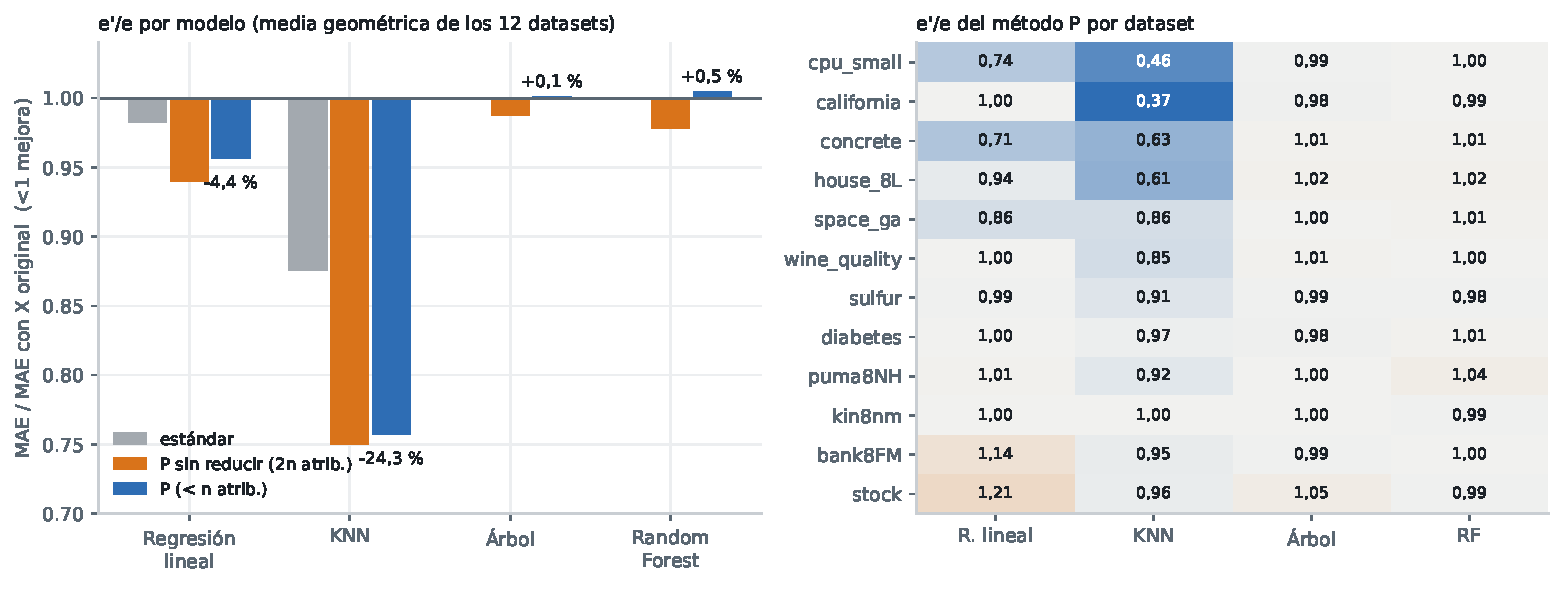
\includegraphics[width=0.9\textwidth]{principal}
\caption{Izquierda: $e'/e$ por modelo para $X$ estandarizado, $P$ sin reducir ($2n$ atributos) y $P$ ($<n$). Derecha: $e'/e$ de $P$ por dataset (azul: mejora; naranja: empeora).}
\label{fig:principal}
\end{figure*}

\begin{table}[htbp]\centering\footnotesize\setlength{\tabcolsep}{2.6pt}
\caption{$e'/e$ (media geométrica de los 12 datasets). \emph{Datasets}: con $e'<e$; $p$: Wilcoxon por dataset con
Holm (8 contrastes); última columna: cambio de $P$ frente a $X$ estandarizado.}
\label{tab:principal}
\begin{tabular}{@{}lcccccc@{}}\toprule
Modelo & estándar & $P$ sin red.\ ($2n$) & $P$ ($<n$) & Datasets & $p$ & vs.\ est.\\\midrule
\filasPrincipal\bottomrule
\end{tabular}
\end{table}

Observamos que en KNN la mejora es grande y significativa, con un \cambioKNN{} frente a la \textit{X} original (p=\pKNN{} en \dsKNN{} datasets), usando menos atributos. Frente a estandarizar, sigue habiendo una reducción significativa con un \cambioVsEstKNN{} (p=\pVsEstKNN). Es decir, seguimos reduciendo el MAE más allá de lo que haría un preprocesado simple. En RL el error baja un \cambioRL{} (\dsRL{} datasets), pero si tenemos en cuenta los 12 datasets y la corrección de Holm, no podemos decir que sea significativo. En el árbol (\cambioArbol) y en RF (\cambioRF) el error se queda igual, así que \textbf{$e'<e$ solo se cumple en media para KNN y RL}. En el peor caso, la RL llega a aumentar el MAE un \peorDsRL{} en uno de los datasets, por lo que nuestro \textit{P} no garantiza mejorar en todos los datasets.

\subsection{La reducción de dimensionalidad}

\begin{table}[htbp]\centering\footnotesize\setlength{\tabcolsep}{4pt}
\caption{Reducción aprendida (media de 5 particiones): $n$ atributos, $s$ conservados, $m$ componentes sintetizadas, $\dim X'=s+m$ y umbral $\tau$ (mediana).}
\label{tab:dimension}
\begin{tabular}{@{}lccccc@{}}\toprule
Dataset & $n$ & $s$ & $m$ & $\dim X'$ & $\tau$\\\midrule
\filasDimension\bottomrule
\end{tabular}
\end{table}

$X'$ usa de media el \dimMedia{} de los atributos y siempre menos de $n$ (\autoref{tab:dimension}): la evolución elimina el \fracEliminados{} de los atributos originales, con un umbral mediano de $\tau=$\tauMediana. En la mayoría de datasets quita uno o dos atributos; en puma8NH, donde pocos atributos explican $y$, se queda con 2 y los complementa con componentes. Frente a $P$ sin reducir ($2n$ atributos), reducir cambia KNN un \cambioRedKNN{} y la RL un \cambioRedRL, sin significación, pero RF empeora un \cambioRedRF{} (p=\pRedRF), porque pierde las $n$ direcciones oblicuas que le daba la síntesis completa. Dentro del presupuesto de $n-1$ atributos, CMA-ES solo sintetiza en el \fracConSintesis{} de las particiones, y quitar la síntesis ($\rho=0$) apenas cambia nada: con un fitness de KNN, el hueco liberado no se aprovecha para dar cortes oblicuos. Por último, si el umbral se fija fuera de la evolución (quitar atributos por peso creciente hasta el menor $s<n$ dentro de un error estándar del mejor fitness), el resultado es parecido (KNN \cribSelKNN); en cambio, un umbral fijo $w_j<0{,}1$ no reduce nada en \cribFijoNoReduce{} particiones. Aprender $\tau$ dentro de la búsqueda cumple siempre el enunciado sin reglas externas.

\subsection{Comparativa con otras transformaciones}
En las mismas particiones comparamos nuestro programa \textit{P} con la estandarización simple, Yeo-Johnson por máxima verosilitud, cuantiles, ''solo PCA'' (sustituir X por sus componentes en el 95\% de varianza o con el \% escogido por validación cruzada), aprendizaje de métricas para regresión (MLKR) y construcción de atributos con programación genética.

\begin{table}[htbp]\centering\footnotesize\setlength{\tabcolsep}{3pt}
\caption{Comparativa: $e'/e$ por modelo (negrita: mejor), $^*$: $P$ es mejor con $p<0{,}05$ (Wilcoxon por dataset,
Holm). Rango: medio de Friedman sobre los cuatro modelos (1 = mejor). $d/n$: $\dim X'$ relativa a $n$.}
\label{tab:comparativa}
\begin{tabular}{@{}lcccccc@{}}\toprule
Transformación & R.\ lin. & KNN & Árbol & RF & Rango & $d/n$\\\midrule
\filasComparativa\bottomrule
\end{tabular}
\end{table}

\begin{figure}[htbp]\centering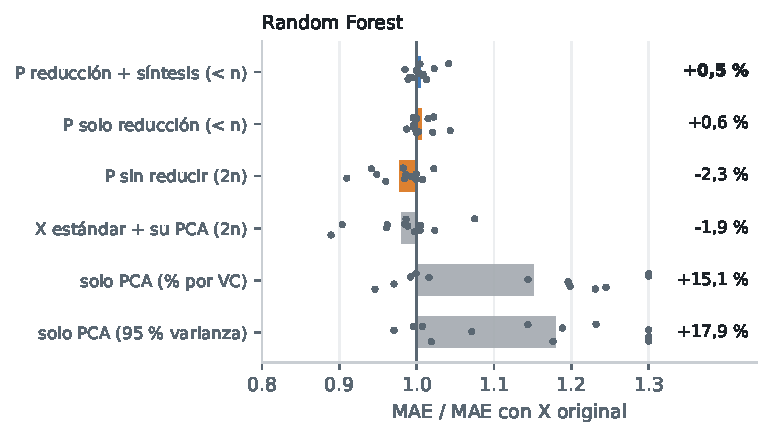
\includegraphics[width=\columnwidth]{sintesis_rf}
\caption{Variantes de síntesis en las mismas particiones (Random Forest). Punto: dataset; barra: media geométrica.}
\label{fig:sintesis}
\end{figure}

\begin{table}[htbp]\centering\footnotesize\setlength{\tabcolsep}{4pt}
\caption{Ablación de la búsqueda: cambio del MAE frente a $P$ (CMA-ES, $m_0=\theta_0$, $\sigma_0=0{,}2$, población por
defecto, $\lambda\in[-2,2]$) en \nAblCasos{} particiones ($>0$: peor que $P$; $^*$: $p<0{,}05$ por dataset, Holm).}
\label{tab:ablacion}
\begin{tabular}{@{}lccc@{}}\toprule
Variante & KNN & R.\ lineal & RF\\\midrule
\filasAblacion\bottomrule
\end{tabular}
\end{table}

\begin{table}[htbp]\centering\footnotesize\setlength{\tabcolsep}{4pt}
\caption{Optimizadores con el mismo $\theta$, fitness y presupuesto (\nAlgCasos{} particiones): rango medio de
fitness (1 = mejor) y cambio del MAE frente a $X$ original.}
\label{tab:algoritmos}
\begin{tabular}{@{}lccc@{}}\toprule
Algoritmo & rango & KNN & R.\ lineal\\\midrule
\filasAlgoritmos\bottomrule
\end{tabular}
\end{table}

\makecontraportada
\end{document}
